\section{The Laplace Equation}

\subsection{Laplace's equation}
Laplace's equation is
\begin{align} \label{eq:5.1}
	\laplacian \phi = 0
\end{align}
This equation describes (among others) steady-state heat flow, potential theory $F = -\grad{\phi}$, and incompressible fluid flow $v = \grad{\phi}$.
The equation \cref{eq:5.1} is solved typically on a domain $D$, where boundary conditions are specified often on the boundary surface.
The Dirichlet boundary conditions fix $\phi$ on the boundary surface $\partial D$.
The Neumann boundary conditions fix $\hat n \cdot \grad{\phi}$ on $\partial D$.

\subsection{Laplace's equation in three-dimensional Cartesian coordinates}
In $\mathbb R^3$ with Cartesian coordinates, Laplace's equation becomes
\begin{align} \label{eq:5.2}
	\pdv[2]{\phi}{x} + \pdv[2]{\phi}{y} + \pdv[2]{\phi}{z} = 0
\end{align}
We seek separable solutions in the usual way:
\begin{align*}
	\phi(x,y,z) = X(x)Y(y)Z(z)
\end{align*}
Substituting,
\begin{align*}
	X''YZ + XY''Z + XYZ'' = 0
\end{align*}
Dividing by $XYZ$ as usual,
\begin{align*}
	\frac{X''}{X} = \frac{-Y''}{Y} - \frac{Z''}{Z} & = -\lambda_\ell \quad \text{(constant)}\\
	\frac{Y''}{Y} = \frac{-Z''}{Z} - \frac{X''}{X} & = -\lambda_m \quad \text{(constant)} \\
	\frac{Z''}{Z} = \frac{-X''}{X} - \frac{Y''}{Y} & = -\lambda_n = \lambda_\ell + \lambda_m
\end{align*}
From the eigenmodes, our general solution will be of the form
\addtocounter{equation}{1}
\begin{align} \label{eq:5.4}
	\phi(x,y,z) = \sum_{\ell,m,n} a_{\ell mn} X_\ell(x) Y_m(y) Z_n(z)
\end{align}

\begin{example}[Steady heat conduction]
    Consider steady ($\pdv{\phi}{t} = 0$) heat flow\footnote{i.e. \cref{eq:4.3} with $\pdv{\phi}{t} = 0$ gives \cref{eq:5.1}} in a semi-infinite rectangular bar, with boundary conditions $\phi = 0$ at $x = 0$, $x = a$, $y = 0$ and $y = b$; and $\phi = 1$ at $z = 0$ and $\phi \to 0$ as $z \to \infty$.
    {\par
    \centering 
    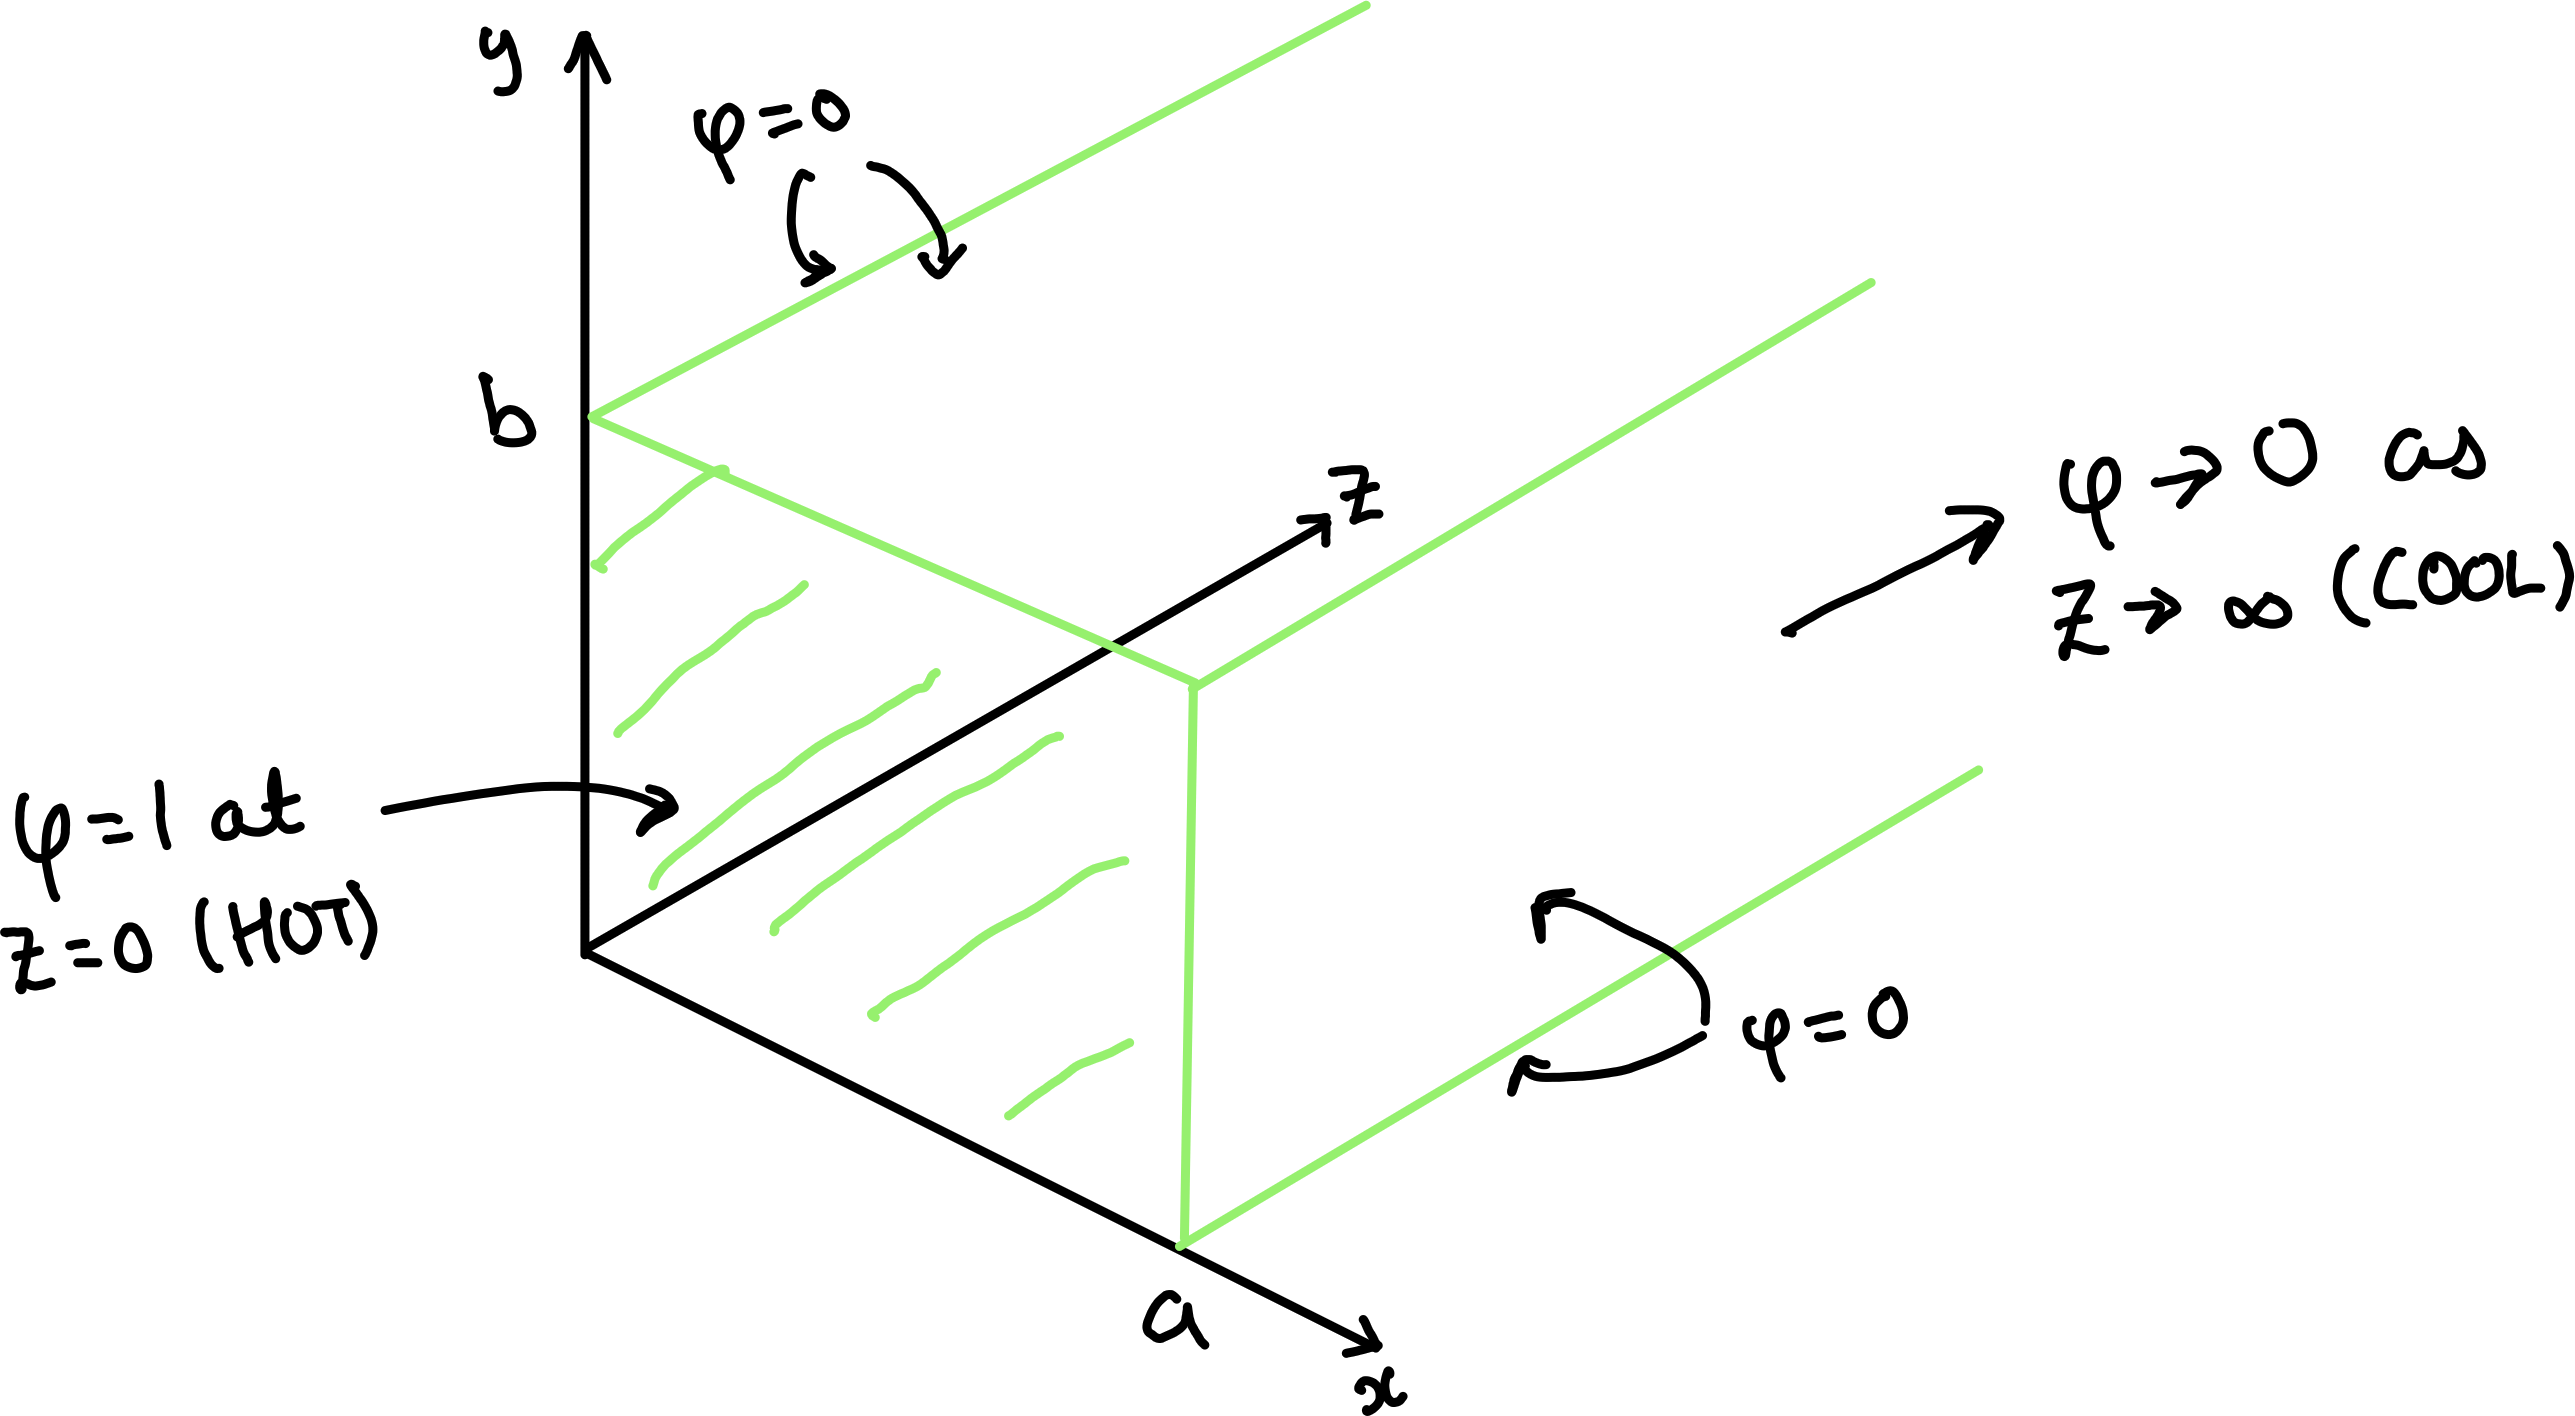
\includegraphics[height=5cm]{05-exm-steadyheat} 
    \par}
    We will solve for each eigenmode successively.
    First, consider $X'' = -\lambda_\ell X$ with $X(0) = X(a) = 0$.
    This gives
    \begin{align*}
        \lambda_\ell = \frac{l^2 \pi^2}{a^2};\quad X_\ell = \sin \frac{\ell \pi x}{a}
    \end{align*}
    where $\ell > 0, \ell \in \mathbb N$.
    By symmetry,
    \begin{align*}
        \lambda_m = \frac{m^2 \pi^2}{b^2};\quad Y_m = \sin \frac{m \pi y}{b}
    \end{align*}
    For the $z$ mode,
    \begin{align*}
        Z'' = -\lambda_n Z = (\lambda_\ell + \lambda_m) Z = \pi^2\qty(\frac{\ell^2}{a^2} + \frac{m^2}{b^2}) Z
    \end{align*}
    Since $\phi \to 0$ as $z \to \infty$, the growing exponentials must vanish.
    Therefore,
    \begin{align*}
        Z_{\ell m} = \exp[-\qty(\frac{\ell^2}{a^2} + \frac{m^2}{b^2})^{1/2} \pi z]
    \end{align*}
    Thus the general solution \cref{eq:5.4} becomes
    \begin{align*}
        \phi(x,y,z) = \sum_{\ell, m} a_{\ell m} \sin \frac{\ell \pi x}{a} \sin \frac{m \pi y}{b} \exp[-\qty(\frac{\ell^2}{a^2} + \frac{m^2}{b^2})^{1/2} \pi z]
    \end{align*}
    Now, we will fix $a_{\ell m}$ using $\phi(x,y,0) = 1$ using the Fourier sine series \cref{eq:1.12}.
    \begin{align*}
        a_{\ell m} = \frac{2}{b} \int_0^b \frac{2}{a} \int_0^a \underbrace{1 \sin \frac{\ell \pi x}{a}}_{\text{square wave}} \underbrace{\sin \frac{m \pi y}{b}}_{\text{square wave}} \dd{x} \dd{y}
    \end{align*}
    So only the odd terms remain, giving
    \begin{align*}
        a_{\ell m} = \frac{4a}{a(2k-1)\pi} \cdot \frac{4b}{b(2p-1) \pi}
    \end{align*}
    where $\ell = 2k-1$ is odd and $m = 2p-1$ is odd.
    Simplifying,
    \begin{align*}
        a_{\ell m} = \frac{16}{\pi^2 \ell m} \quad \text{ for } \ell, m \text{ odd}
    \end{align*}
    So the heat flow solution is
    \begin{align*}
        \phi(x,y,z) = \sum_{\ell, m \text{ odd}} \frac{16}{\pi^2 \ell m} \sin \frac{\ell \pi x}{a} \sin \frac{\ell \pi y}{b} \exp[-\qty(\frac{\ell^2}{a^2} + \frac{m^2}{b^2})^{1/2} \pi z]
    \end{align*}
    As $z$ increases, every contribution but the lowest mode will be very small.
    So low $\ell, m$ dominate the solution.

    Cross sectionals:
    insertpicture
\end{example} 

\subsection{Laplace's equation in plane polar coordinates}
In plane polar coordinates, Laplace's equation becomes
\addtocounter{equation}{1}
\begin{align} \label{eq:5.6}
	\frac{1}{r} \pdv{r} \qty(r \pdv{\phi}{r}) + \frac{1}{r^2} \pdv[2]{\phi}{\theta} = 0
\end{align}
Consider a separable form of the answer, given by
\begin{align*}
	\phi(r,\theta) = R(r) \Theta(\theta)
\end{align*}
We then have
\begin{align*}
	\Theta'' + \mu \Theta = 0;\quad r(rR')' - \mu R = 0
\end{align*}

\subsubsection{Polar equation}
The polar equation can be solved easily by considering periodic boundary conditions.
This gives $\mu = m^2$ and the eigenmodes as in \cref{eq:3.25}
\begin{align*}
	\Theta_m(\theta) = \cos m \theta, \sin m \theta
\end{align*}

\subsubsection{Radial equation}
The radial equation is \textit{not} Bessel's equation, since there is no second separation constant.
We simply have
\begin{align} \label{eq:5.7}
	r(rR')' - m^2 R = 0
\end{align}
We will try a power law solution, $R = \alpha r^\beta$.
We find
\begin{align*}
	\beta^2 - m^2 = 0 \implies \beta = \pm m
\end{align*}
So the eigenfunctions are
\begin{align*}
	R_m(r) = r^m, r^{-m}
\end{align*}
which is one regular solution at the origin and one singular solution. \\
In the case $m = 0$, we have
\begin{align*}
	(rR')' = 0 \implies rR' = \text{constant} \implies R = \log r
\end{align*}
So
\begin{align*}
	R_0(r) = \text{constant or } \log r
\end{align*}
The general solution is therefore
\begin{align} \label{eq:5.8}
	\phi(r,\theta) = \frac{a_0}{2} + c_0 \log r + \sum_{m=1}^\infty \qty(a_m \cos m\theta + b_m \sin m\theta) r^m + \sum_{m=1}^\infty \qty(c_m \cos m\theta + d_m \sin m\theta) r^{-m}
\end{align}

\begin{example}[Soap Film on a Unit Disc]
    insertpicture

	Consider a soap film on a unit disc.
	We wish to solve Laplace's equation \cref{eq:5.6} with a vertically distorted circular wire of radius $r = 1$ with boundary conditions $\phi(1, \theta) = f(\theta)$.
	The $z$ displacement of the wire produces the $f(\theta)$ term.
	We wish to find $\phi(r,\theta)$ for $r < 1$, assuming regularity at $r = 0$.
	Then, $c_m = d_m = 0$ and so \cref{eq:5.8} becomes
	\begin{align*}
		\phi(r,\theta) = \frac{a_0}{2} + \sum_{m=1}^\infty \qty(a_m \cos m\theta + b_m \sin m\theta) r^m
	\end{align*}
	At $r = 1$,
	\begin{align*}
		\phi(1,\theta) = f(\theta) = \frac{a_0}{2} + \sum_{m=1}^\infty \qty(a_m \cos m\theta + b_m \sin m\theta)
	\end{align*}
	which is exactly the Fourier series.
	Thus by \cref{eq:1.5},
	\begin{align*}
		a_m = \frac{1}{\pi} \int_0^{2\pi} f(\theta) \cos m \theta \dd{\theta};\quad b_m = \frac{1}{\pi} \int_0^{2\pi} f(\theta) \sin m \theta \dd{\theta}
	\end{align*}
	We can see from the equation that high harmonics are confined to have effects only near $r = 1$.
\end{example}

\begin{figure}[h] 
    \centering 
    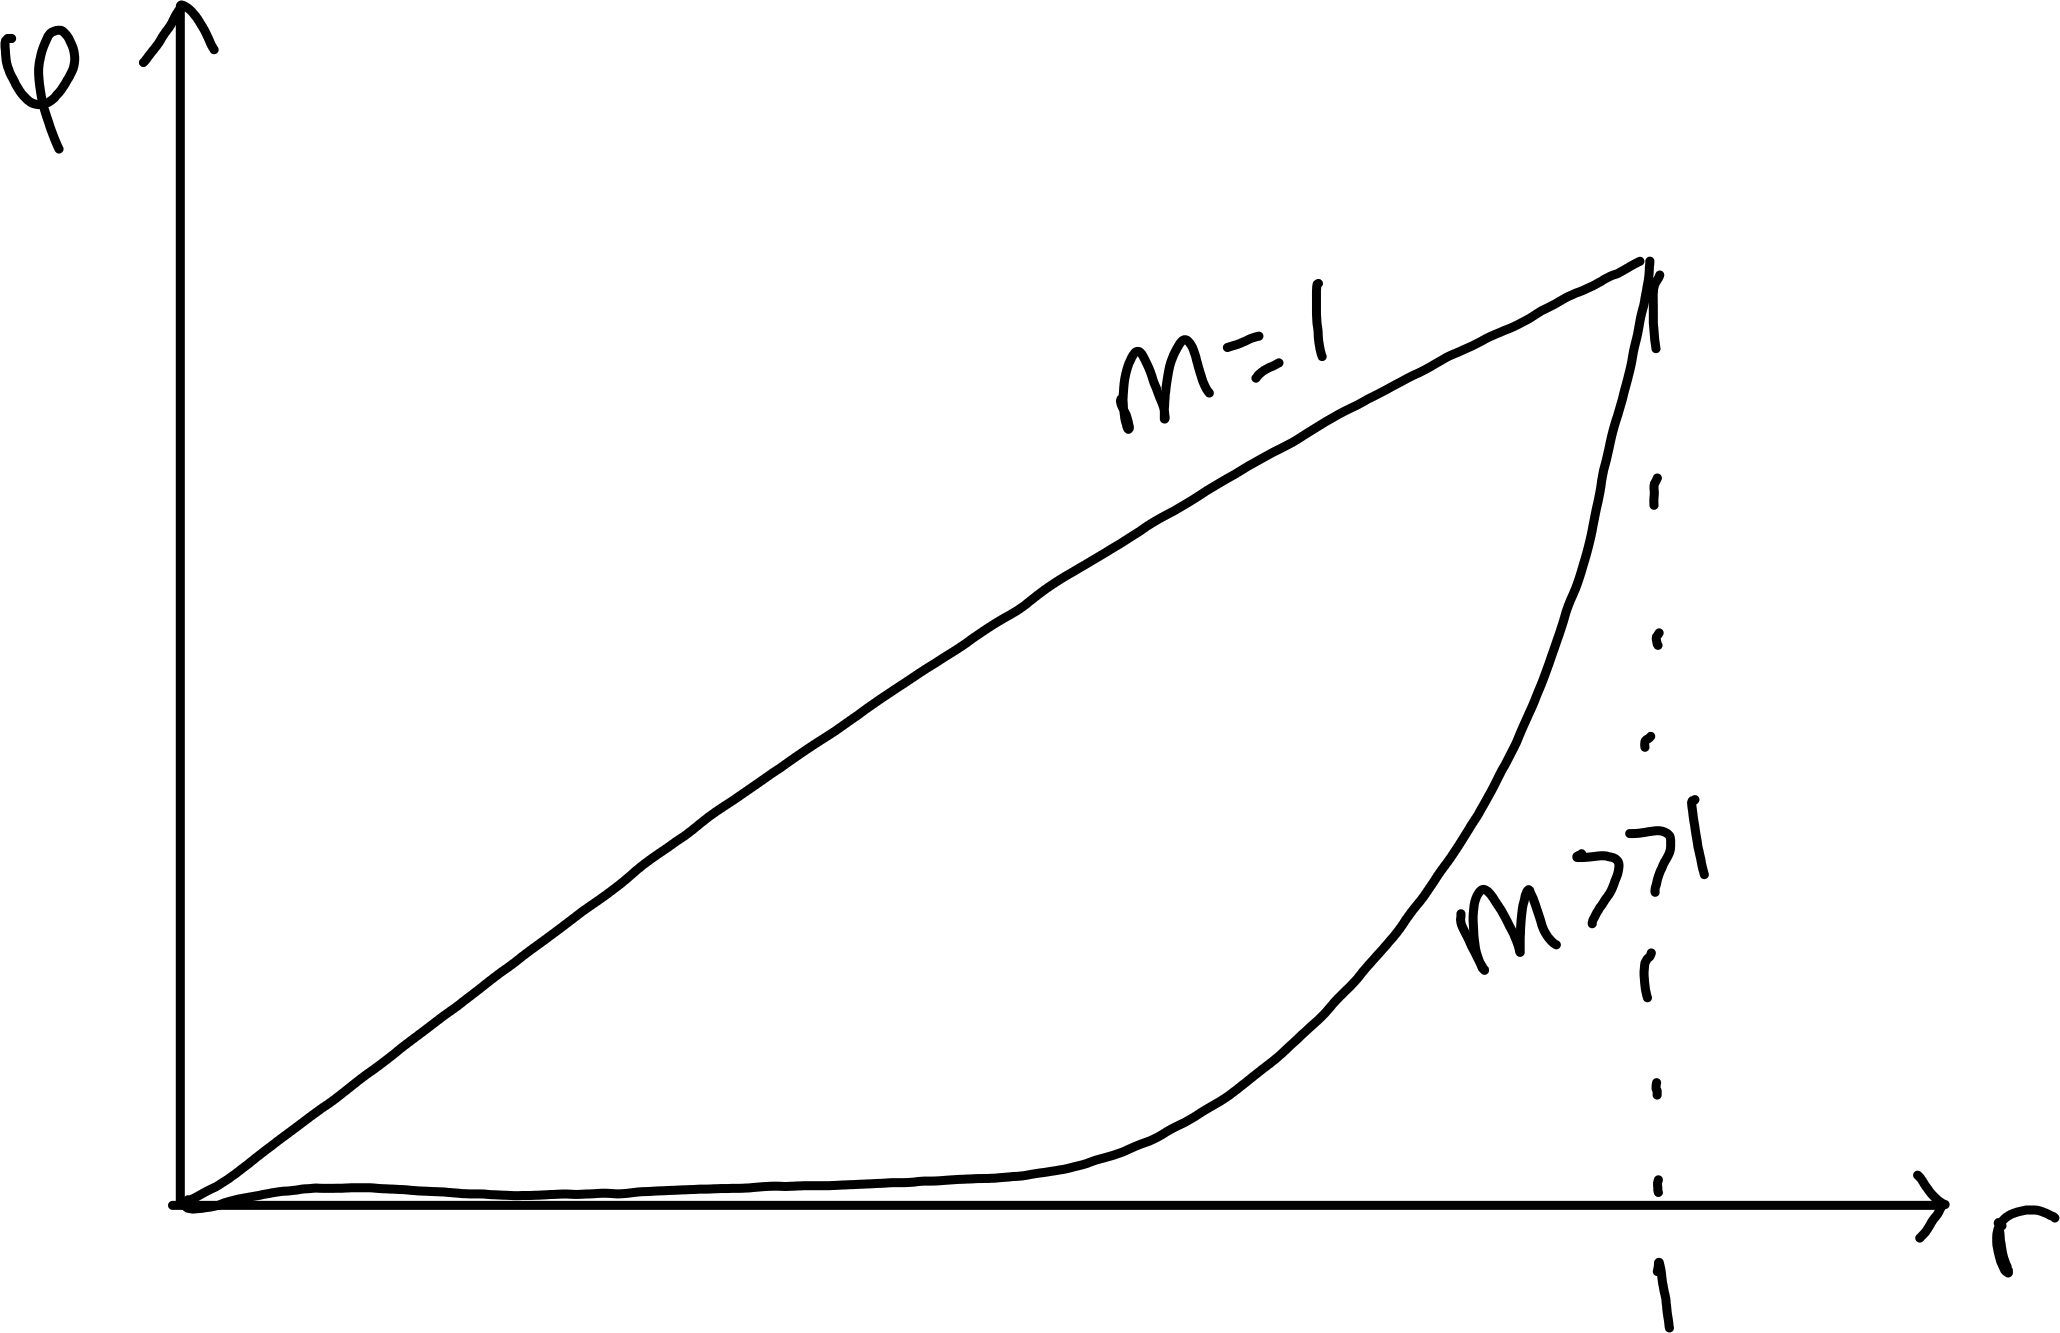
\includegraphics[height=5cm]{05-polarsoln} 
\end{figure}

\subsection{Laplace's equation in cylindrical polar coordinates}
In cylindrical coordinates,
\begin{align*}
	\frac{1}{r} \pdv{r} \qty(r \pdv{\phi}{r}) + \frac{1}{4^2} \pdv[2]{\phi}{\theta} + \pdv[2]{\phi}{z} = 0
\end{align*}
With $\phi = R(r) \Theta(\theta) Z(z)$, we find
\begin{align*}
	\Theta'' = -\mu \Theta;\quad Z'' = \lambda Z;\quad r(rR')' + (\lambda r^2 - \mu) R = 0
\end{align*}
The polar equation can be easily solved by
\begin{align*}
	\mu_m = m^2;\quad \Theta_m(\theta) = \cos m\theta, \sin m\theta
\end{align*}
The radial equation is Bessel's equation, giving solutions
\begin{align*}
	R = J_m(kr), Y_m(kr)
\end{align*}
Setting boundary conditions in the usual way, defining $R=0$ at $r = a$ means that
\begin{align*}
	J_m(ka) = 0 \implies k = \frac{j_{mn}}{a}
\end{align*}
The radial solution is
\begin{align*}
	R_{mn}(r) = J_m\qty(\frac{j_{mn}}{a}r)
\end{align*}
We have eliminated the $Y_n$ term since we require $r = 0$ to give a finite $\phi$.
Finally, the $z$ equation gives
\begin{align*}
	Z'' = k^2 Z \implies Z = e^{-kz}, e^{kz}
\end{align*}
We typically eliminate the $e^{kz}$ mode due to boundary conditions, such as $Z \to 0$ as $z \to \infty$.
The general solution is therefore
\begin{align*}
	\phi(r,\theta,z) = \sum_{m=0}^\infty \sum_{n = 1}^\infty \qty(a_{mn} \cos m\theta + b_{mn} \sin m\theta) J_m\qty(\frac{j_{mn}}{a} r) e^{-frac{j_{mn}r}{a}}
\end{align*}

\subsection{Laplace's equation in spherical polar coordinates}
In spherical polar coordinates,
\begin{align*}
	\frac{1}{r^2} \pdv{r} \qty(r^2 \pdv{\Phi}{r}) + \frac{1}{r^2 \sin\theta}\pdv{\theta} \qty(\sin\theta \pdv{\Phi}{\theta}) + \frac{1}{r^2 \sin^2 \theta} \pdv[2]{\Phi}{\phi} = 0
\end{align*}
We will consider the \textit{axisymmetric case}; supposing that there is no $\phi$ dependence.
We seek a separable solution of the form
\begin{align*}
	\Phi(r,\theta) = R(r) \Theta(\theta)
\end{align*}
which gives
\begin{align*}
	(\sin\theta \Theta')' + \lambda \sin\theta \Theta = 0;\quad (r^2R')' - \lambda R = 0
\end{align*}
Consider the substitution $x = \cos\theta, \dv{x}{\theta} = -\sin\theta$ in the polar equation.
This gives $\dv{\Theta}{\theta} = -\sin\theta \dv{\Theta}{x}$ and hence
\begin{align*}
	-\sin\theta \dv{x}\qty[-\sin^2\theta \dv{\Theta}{x}] + \lambda \sin\theta \Theta = 0 \implies \dv{x}\qty[(1-x^2)\dv{\Theta}{x}] + \lambda \Theta = 0
\end{align*}
This gives Legendre's equation, so it has solutions of eigenvalues $\lambda_\ell = \ell (\ell + 1)$ and eigenfunctions
\begin{align*}
	\Theta_\ell(\theta) = P_\ell(x) = P_\ell(\cos\theta)
\end{align*}
The radial equation then gives
\begin{align*}
	(r^2 R')' - \ell (\ell + 1) R = 0
\end{align*}
We will seek power law solutions: $R = \alpha r^\beta$.
This gives
\begin{align*}
	\beta(\beta + 1) - \ell(\ell + 1) = 0 \implies \beta = \ell, \beta = -\ell - 1
\end{align*}
Thus the radial eigenmodes are
\begin{align*}
	R_\ell = r^{\ell}, r^{-\ell - 1}
\end{align*}
Therefore the general axisymmetric solution for spherical polar coordinates is
\begin{align*}
	\Phi(r,\theta) = \sum_{\ell = 0}^\infty (a_\ell r^{\ell} + b_\ell r^{-\ell - 1}) P_\ell(\cos\theta)
\end{align*}
The $a_\ell, b_\ell$ are determined by the boundary conditions.
Orthogonality conditions for the $P_\ell$ can be used to determine coefficients.
Consider a solution to Laplace's equation on the unit sphere with axisymmetric boundary conditions given by
\begin{align*}
	\Phi(1,\theta) = f(\theta)
\end{align*}
Given that we wish to find the interior solution, $b_n = 0$ by regularity.
Then,
\begin{align*}
	f(\theta) = \sum_{\ell=0}^\infty a_\ell P_\ell(\cos\theta)
\end{align*}
By defining $f(\theta) = F(\cos\theta)$,
\begin{align*}
	F(x) = \sum_{\ell=0}^\infty a_\ell P_\ell(x)
\end{align*}
We can then find the coefficients in the usual way, giving
\begin{align*}
	a_\ell = \frac{2\ell + 1}{2} \int_{-1}^1 F(x) P_{\ell}(x) \dd{x}
\end{align*}

\subsection{Generating function for Legendre polynomials}
Consider a charge at $r_0 = (x,y,z) = (0,0,1)$.
Then, the potential at a point $P$ becomes
\begin{align*}
	\Phi(r) & = \frac{1}{\abs{r - r_0}} = \frac{1}{(x^2 + y^2 + (x-1)^2)^{1/2}} \\
	& = \frac{1}{(r^2 (\sin^2 \phi + \cos^2 \phi) \sin^2 \theta + r^2 \cos^2 \theta - 2r \cos\theta + 1)^{1/2}} \\
	& = \frac{1}{(r^2 \sin^2 \theta + r^2 \cos^2 \theta - 2r \cos\theta + 1)^{1/2}} \\
	& = \frac{1}{(r^2 - 2r \cos\theta + 1)^{1/2}} \\
	& = \frac{1}{(r^2 - 2r \overline x + 1)^{1/2}}
\end{align*}
where 

$\overline x \equiv \cos \theta$.
This function $\Phi$ is a solution to Laplace's equation where $r \neq r_0$.
Note that we can represent any axisymmetric solution as a sum of Legendre polynomials.
Now,
\begin{align*}
	\frac{1}{\sqrt{r^2 - 2rx + 1}} = \sum_{\ell = 0}^\infty a_\ell P_\ell(x) r^\ell
\end{align*}
With the normalisation condition for the Legendre polynomials $P_\ell(1) = 1$, we find
\begin{align*}
	\frac{1}{1-r} = \sum_{\ell=0}^\infty a_\ell r^\ell
\end{align*}
Using the geometric series expansion, we arrive at $a_\ell = 1$.
This gives
\begin{align*}
	\frac{1}{\sqrt{r^2 - 2rx + 1}} = \sum_{\ell = 0}^\infty P_\ell(x) r^\ell
\end{align*}
which is the generating function for the Legendre polynomials.